\begin{figure}[h]
    \centering
    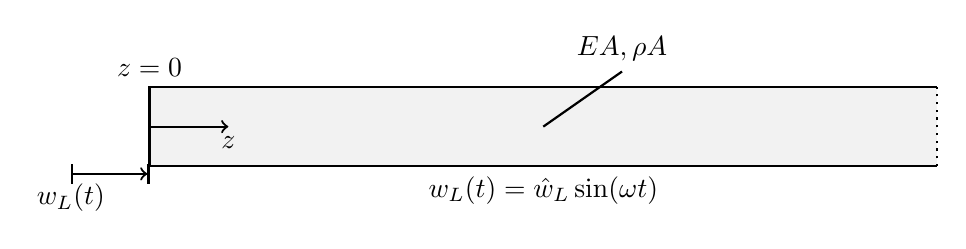
\begin{tikzpicture}
        \draw[thick, fill=gray!10] (10,0) -- node [midway, below] {$w_L (t) = \hat{w}_L \sin(\omega t)$} (0,0) -- (0,1) node[above] {$z=0$} -- (10,1) ;
        \draw[thick, dotted] (10,0) -- (10,1);
        %\draw[thick, ->] (10,0.5) -- (11,0.5);
        \draw[thick, ->] (0,0.5) -- (1,0.5) node[left, below] {$z$} ;
        \draw[thick, |->|] (-1,-0.1) node[below] {$w_L (t)$} -- (0,-0.10);
        \draw[thick] (5,0.5) -- (6,1.2) node[above] {$EA,\rho A$};
    \end{tikzpicture}
\end{figure}
